\section{ECAs as Discrete Maps}

As shown in section 2, ECAs that are allowed to grow infinitely in size can exhibit non-periodic and chaotic behavior, even though they are completely deterministic.   
In this section we will only consider CAs with a fixed number of cells.  
For this case, we must apply either fixed or periodic boundary conditions on the endpoints.  
In this work we use periodic boundary conditions and the space transforms from an infinite 1D lattice into a finite circular lattice.  
For an ECA of finite width, $n$, there exists $2^n$ possible configurations (each site takes one of two values).  
This means that every initial condition will eventually end in a periodic loop, although the period could be as large as $2^n$.  

\subsection{Converting Rules Into Maps}

We follow the methods of~\cite{sed} to convert the graphical ECA rules into discrete 1D maps.  
In the same way each rule is labeled by a binary number, each time step in our finite ECA may be converted from binary into a base-10 number.  
We wrote a \textsc{C++} code to loop over all $2^n$ possible configurations and record the resulting configuration after applying the ECA rule (both are recorded in base 10).  
Compiling all this information together, we get a 1D discrete map, mapping all the integers [0, $2^n -1$] $\rightarrow$ [0, $2^n -1$] for a given ECA rule.  
The resulting maps are shown in Figures~\ref{30map} and~\ref{126map}.  
The densely filled area is a result of lines connecting all successive points in the map.  
Figure~\ref{30map_dot} shows the same figure without the  lines connecting successive points.  
We can now iterate this mapping, using either cobweb diagrams or computer routines, to see the evolution of ECA over each time step.  

\begin{figure}
    \begin{minipage}[b]{0.49\textwidth}
        \centering
        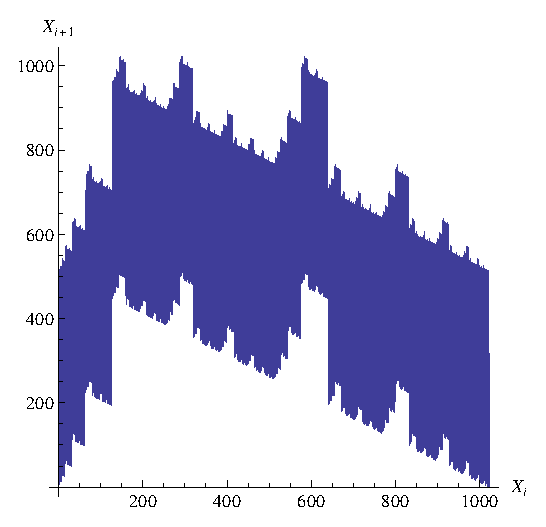
\includegraphics[width=\textwidth]{30map.eps}
        \caption{\label{30map} The mapping for rule 30, using a grid width of 10 lattice points.  }
    \end{minipage}
    \hspace{0.5cm}
    \begin{minipage}[b]{0.49\textwidth}
        \centering
        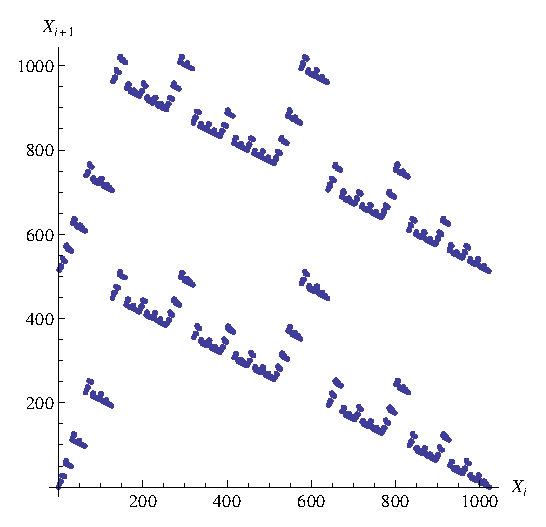
\includegraphics[width=\textwidth]{30map_dot.eps}
        \caption{\label{30map_dot} Figure~\ref{30map}, shown without lines connecting successive points.}
    \end{minipage}
\end{figure}

The resulting maps are much more complicated in appearance than any of the maps we studied during the semester, such as the chaotic logistic map.  
The maps studied here have descrete values along the axes, where as the logistic map is continuous, so there is no possibility of rounding error or computer dependent results.  
Adding more lattice points to the map results in the same structure, but with a higher resolution.  
This is shown in Figures~\ref{126map_6} and~\ref{126map} where the lattice size is varied from six to ten points.  
Figure~\ref{126map_6} illustrates how rapid oscillations between two values leads to the filled in region.  
The two values differ by 512, or one bit, and demonstrate how changing one bit can lead to a very different response.   

\begin{figure}
    \begin{minipage}[b]{0.49\textwidth}
        \centering
        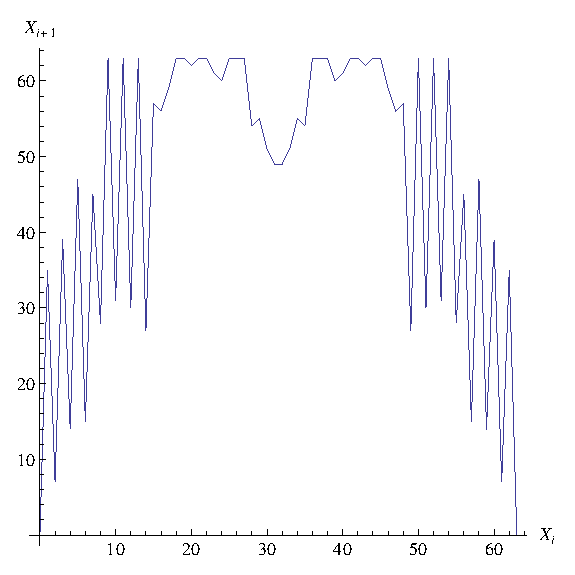
\includegraphics[width=\textwidth]{126map_6.eps}
        \caption{\label{126map_6} The mapping for rule 126 using a width of 6 lattice points.  }
    \end{minipage}
    \hspace{0.5cm}
    \begin{minipage}[b]{0.49\textwidth}
        \centering
        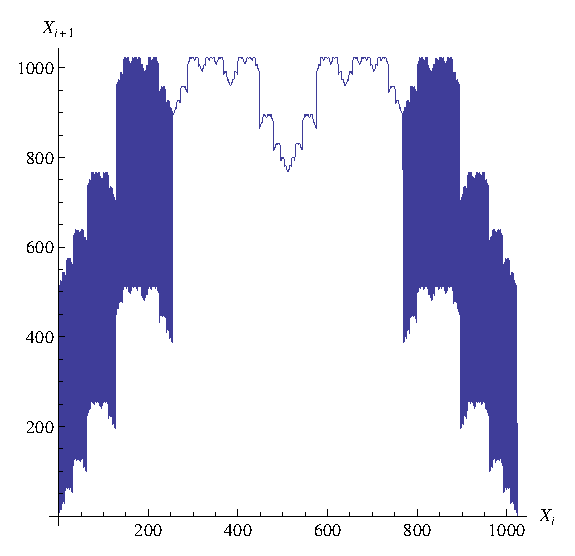
\includegraphics[width=\textwidth]{126map.eps}
        \caption{\label{126map} The mapping for rule 126 using a width of 10 lattice points.}
    \end{minipage}
\end{figure}

\subsection{Dependence on Initial Conditions}

By iterating these maps we can look at the growth of the system as a function of time step.  As previously mentioned, all initial conditions will eventually reach a periodic cycle.  Figure~\ref{30iter_IC32} shows the growth of rule 30 over 1,000 iterations with an initial condition of 32 (one black block).  This system hits a stable period-15 cycle after 7 iterations.  Figure~\ref{30iter_IC33} shows the same evolution of rule 30, but now with an initial condition of 33.  These two initial conditions only differ by one bock, but the system now hits a period-5 cycle immediately after starting.  

Figure~\ref{30iter_IC34} once again shows rule 30 over 1,000 time steps, now with an initial value of 34.  Bit wise, the initial condition of 34 differs by only one cell from 32, and has two adjacent cells swapped from 33.  We can see that the initial value 34 takes slightly longer (25 iterations) but also settles on a period-15 cycle.  This period-15 cycle, however, is completely different from the period-15 cycle produced by starting condition 32.  Even though the initial conditions may not be continuously varied in these discrete systems, a strong sensitivity to initial conditions is still present.  

\begin{figure}
    \begin{minipage}[b]{0.49\textwidth}
        \centering
        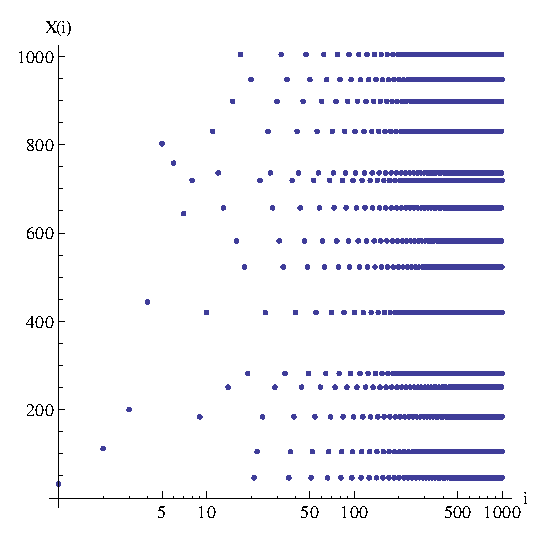
\includegraphics[width=\textwidth]{30iter_IC32.eps}
        \caption{\label{30iter_IC32} 1,000 iterations of rule 30 with an initial value of 32.   }
    \end{minipage}
    \hspace{0.5cm}
    \begin{minipage}[b]{0.49\textwidth}
        \centering
        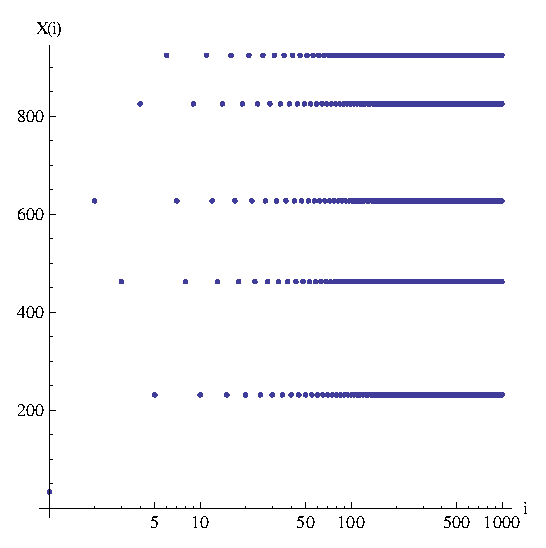
\includegraphics[width=\textwidth]{30iter_IC33.eps}
        \caption{\label{30iter_IC33} 1,000 iterations of rule 30 using the initial value 33. }
    \end{minipage}
\end{figure}

\begin{figure}
    \begin{minipage}[b]{0.49\textwidth}
        \centering
        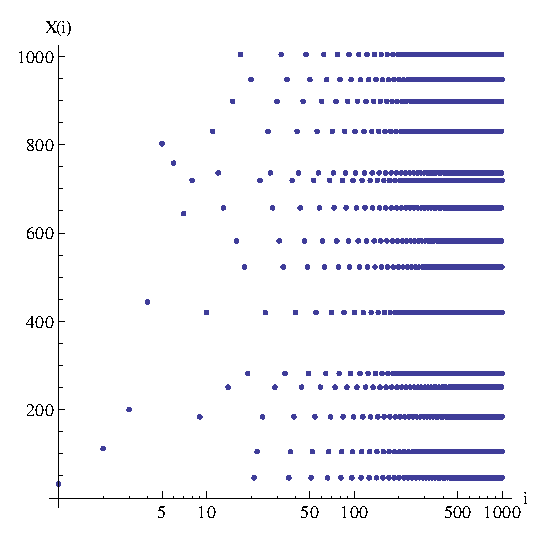
\includegraphics[width=\textwidth]{30iter_IC32.eps}
        \caption{\label{30iter_IC32_2} 1,000 iterations of rule 30 with an initial value of 32.   }
    \end{minipage}
    \hspace{0.5cm}
    \begin{minipage}[b]{0.49\textwidth}
        \centering
        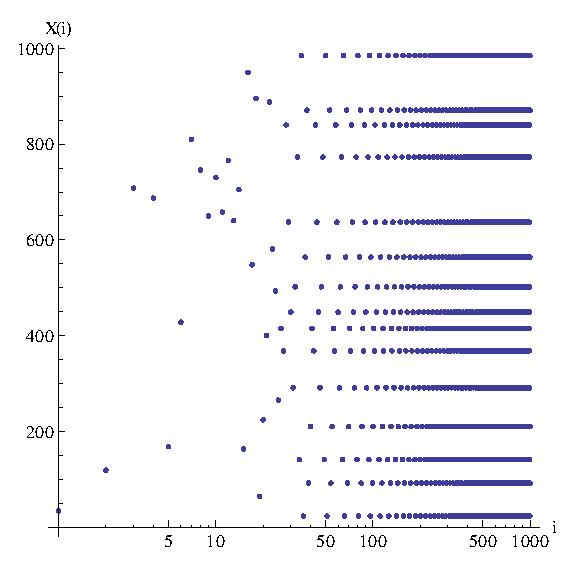
\includegraphics[width=\textwidth]{30iter_IC34.eps}
        \caption{\label{30iter_IC34} 1,000 iterations of rule 30 using the initial value 34. }
    \end{minipage}
\end{figure}

We can run our code for all initial values from 0 to $2^n$ and plot the resulting limit cycle.  This information is plotted in Figure~\ref{30bif} for rule 30 and Figure~\ref{126bif} for rule 126.  From these plots it can be seen that there is a high variability in which limit cycle results from different initial conditions.  There is an interesting trend where bands of states do not appear in any of the possible limit cycles.  

\begin{figure}
    \begin{minipage}[b]{0.49\textwidth}
        \centering
        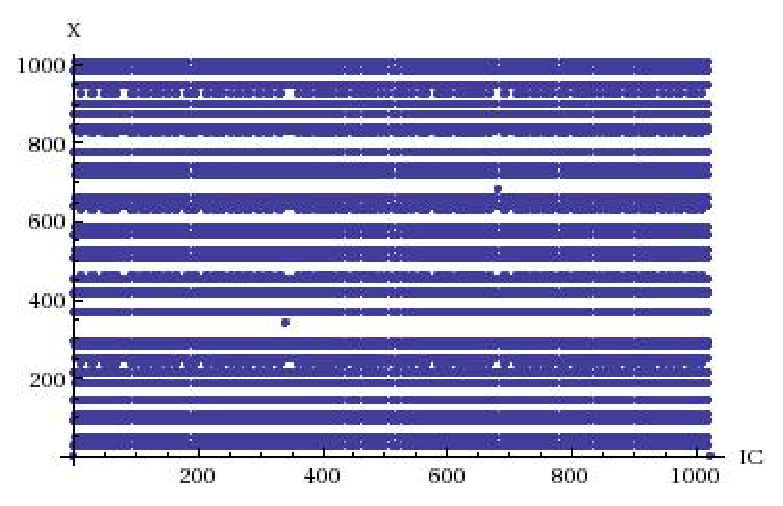
\includegraphics[width=\textwidth]{30bif.eps}
        \caption{\label{30bif} The limit cycles of rule 30, plotted as a function of all initial conditions [0, 1023]}
    \end{minipage}
    \hspace{0.5cm}
    \begin{minipage}[b]{0.49\textwidth}
        \centering
        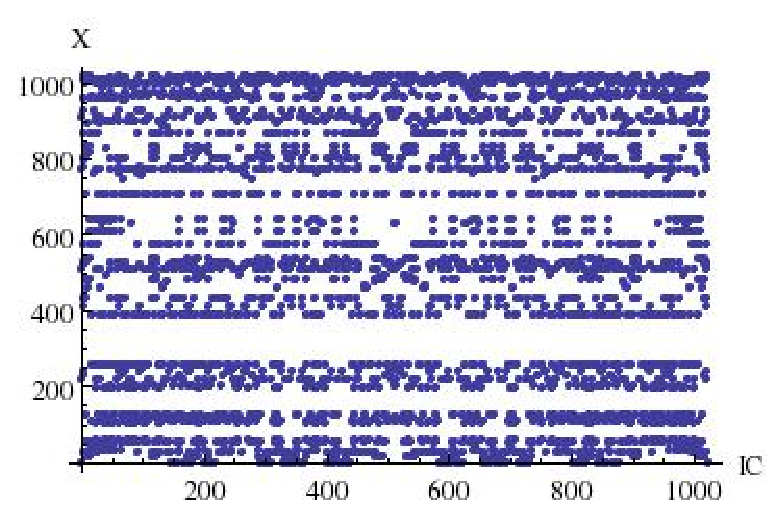
\includegraphics[width=\textwidth]{126bif.eps}
        \caption{\label{126bif} The limit cycles of rule 126, plotted as a function of all initial conditions [0, 1023] }
    \end{minipage}
\end{figure}

\subsection{Fractal Dimension}

Many of the ECA rules result in fractal patterns.  The easiest way to classify these patters is by their fractal dimension.  The fractal dimension is given by:
\begin{equation}
	D = - \frac{\log N}{\log \epsilon},
\end{equation}
where N is the number of new branches per iteration and $\epsilon$ is the scaling factor for each branch.  The fractal image produced by rule 126, shown in Figure~\ref{rule126}, has N = 3 branches per iteration and a scaling factor of $\epsilon$ = 0.5.  This results in a fractal dimension of $\log 3/\log 2 \approx 1.58$.  Interestingly, the map version of rule 126 also shows repeating shapes with a scaling factor of 0.5 and, although hard to see, three branches per iteration.  This would give the map the exact same fractal dimension as the Sierpinski triangle pattern that it creates.  It should be noted that this argument is only valid as the number of lattice points goes to infinity; the map is one dimensional for a finitely sized lattice.  
